% This LaTeX was auto-generated from MATLAB code.
% To make changes, update the MATLAB code and export to LaTeX again.

\documentclass{article}

\usepackage[utf8]{inputenc}
\usepackage[T1]{fontenc}
\usepackage{lmodern}
\usepackage{graphicx}
\usepackage{color}
\usepackage{hyperref}
\usepackage{amsmath}
\usepackage{amsfonts}
\usepackage{epstopdf}
\usepackage[table]{xcolor}
\usepackage{matlab}

\sloppy
\epstopdfsetup{outdir=./}
\graphicspath{ {./seguimiento5_images/} }

\begin{document}

\matlabtitle{Seguimiento N°5}

\begin{par}
\begin{flushleft}
Nombre: Valentina Andrade de la Horra
\end{flushleft}
\end{par}

\begin{par}
\begin{flushleft}
Ayudantes: Pablo Vega y Bianca Hincapié
\end{flushleft}
\end{par}

\begin{par}
\begin{flushleft}
Primero corremos el codigo que permite obtener la trayectoria del consumo. Para ello utilizamos dos funciones: crra.m (que contiene la funcion de utilidad CRRA) y value\_matrix.m (material entregado en ayudantía)
\end{flushleft}
\end{par}

\begin{matlabcode}
%% Consumo en el ciclo de vida - item (a)
clc; clear; close all;

%Parameters
T =65; 
beta = 0.96; 
sigma = 2; 
r = 0.04; 
liq = 100;
A = linspace(-15,25,1001)'; % Tienen como deuda maxima -15 y ahorro 25
% Si mi restriccion de liquidez es b = 100 no es activo

%Wage as function and vector
Z  = @(t) 1.25 + 6e-2*t - 1e-3*t.^2; % se multiplica escalar, entonces voy a ocupar vectores
w = Z(1:T); % evaluar desde 1 hasta t
w_mean = mean(w)*ones(1,T); % ones es para hacer un vector de la media

%Value function iteration
tic
[~,~,Ct,~,~,~] = value_matriz(T,beta,sigma,r,A,Z,liq);
toc
\end{matlabcode}
\begin{matlaboutput}
Elapsed time is 0.539746 seconds.
\end{matlaboutput}

\matlabheadingthree{(a) Obtenga la ecuación de Euler del agente e interprete}

\begin{par}
$$u^{\prime } \left(c_t \left(1+e_t \right)\right)=\beta \;{\mathrm{Ru}}^{\prime } \left(c_{t+1} \;\right)\;\;\;\;\;\;\;\;\;\;\;\;\;\;\;\;\;\left(1\right)$$    
\end{par}

\begin{par}
\begin{flushleft}
Recordemos que la forma funcional de la utilidad, dado que $\sigma =2$, es la siguiente
\end{flushleft}
\end{par}

\begin{par}
$$\frac{c^{1-\sigma \;} -1}{1-\sigma }\longrightarrow \frac{\partial \;\frac{\left(c^{1-\sigma } -1\right)}{1-\sigma }}{\partial \;c}=c^{-\sigma }$$
\end{par}

\begin{par}
\begin{flushleft}
Luego de (1) podemos pontener que
\end{flushleft}
\end{par}

\begin{par}
\begin{flushleft}
${\left(c_{t\;} \;\left(1+e_t \right)\right)}^{-\sigma } =\beta {{\mathrm{Rc}}_{t+1} }^{-\sigma } \;$´   (2)
\end{flushleft}
\end{par}

\begin{par}
$$\frac{{\left(c_{t\;} \;\left(1+e_t \right)\right)}^{-\sigma } }{{c_{t+1} }^{-\sigma } \;}=\beta R$$
\end{par}

\begin{par}
\begin{flushleft}
Aplicando $-\frac{1}{\sigma }$ y despejando el error 
\end{flushleft}
\end{par}

\begin{par}
\begin{flushleft}
$\;{e_t } ={\left(\beta R\right)}^{-\frac{1}{\sigma }} \;\cdot {\frac{c_{t+1} }{c_t }} -1$ (3)
\end{flushleft}
\end{par}

\begin{par}
\begin{flushleft}
Interpretación: Si tomamos la ecuación (2) notaremos que el costo marginal de consumir hoy respecto al retorno marginal de consumir mañana, está descontado por la impaciencia del consumo actual y los retornos que otorga la tasa de interés. Además, si bien tenemos una tasa de sustitución intertemporal $-\sigma \;$ (que nos da una medida de la capacdad de respuesta de la tasa de crecimiento del consumo a la tasa de interés real, es decir, cómo cambia el consumo presente ante cambios en el futuro), podemos notar que esta es igual para las utilidades marginales. Ahora bien, si tienen implicancias para el $\beta R$. Por ejemplo, si suben los tipos reales, el consumo futuro puede aumentar debido a la mayor rentabilidad de los ahorros, pero el consumo futuro tambien puede disminuir a medida que el "ahorrador" decide consumir menos teniendo en cuenta que puede conseguir un amyor retorno de lo que ahorra (es decir, consume). El efecto neto de esta relación sobre el futuro es capturado por este $-\frac{1}{\sigma }$ que es la elasticidad de sustitución intertemporal. Ahora bien, despejando esos elementos que ya conocíamos, podemos notar que aparece un elemento relevante en este análisis del trade off que expresa la ecuación de Euler. 
\end{flushleft}
\end{par}

\begin{par}
\begin{flushleft}
Si miramos la ecuación (3) notaremos que existe un error asociado a esa relación que establece el consumo futuro y el consumo actual, \textbf{ponderado por ese factor psicológico de impaciencia y ese factor económico de retornos de las tasas (con una elasticidad que ya comentamos). }Es decir, pese a que obtenemos una medida para entender como el agente suaviza consumo en dos periodos, este está sujeto a un error y este error es estocástico ($\left.e_t \right)$. Es decir, del total del consumo (por eso aparece el -1), si tomo la relación entre el consumo mañana y hoy, existe un elemento que no logra explicar los factores que hemos \textbf{medido }y determinado. 
\end{flushleft}
\end{par}

\begin{par}
\begin{flushleft}
Una nota importante es que ese error no tiene que ver con el consumo futuro, sino que con el consumo actual. A mi parecer la razón yace en que, en general, los problemas de consumo en horizonte finito se resuelven tomando como dados el último periodo y luego resolvemos la decisión del agente hacia el consumo anterior. Es decir, en\textit{ t+1 }(último periodo) tenemos certeza sobre qué determina el consumo: si me queda algo por consumir me lo consumo todo. Dado eso, elijo mi consumo en \textit{t.} Y en esa estimación tendremos un error. Ahora bien, como veremos en (b) ese error es aleatorio, y como visualizaremos numéricamente más adelante su valor esperado será cercano a cero. 
\end{flushleft}
\end{par}

\matlabheadingthree{(b) Representación de los errores}

\begin{par}
\begin{flushleft}
Luego, calculemos los errores con una iteración que traduce (3) en una iteración. Concretamente lo que haremos es calcular un error para cada periodo, en base a la relación antes descrita. 
\end{flushleft}
\end{par}

\begin{matlabcode}
constant=(beta*(1+r))^(-1/sigma);
errors=zeros(1,T);
for k=1:T-1    
    errors(k)=constant*(Ct(k+1))/Ct(k)-1;
end
\end{matlabcode}

\begin{par}
\begin{flushleft}
En el siguiente gráfico mostraremos la distribución en el tiempo de los errores, pero además mostraremos dos momentos de la distribución de este error: su media y su varianza. 
\end{flushleft}
\end{par}

\begin{matlabcode}
tx= {'Interpreter','Latex','FontSize', 15};
meanVal = mean(errors);
stdVal = std(errors);
str = sprintf('Mean: %f\n Std: %f',meanVal,stdVal);

figure(1)
plot(1:T, errors(:,1:end))
yline(0,'LineStyle','-.','Label','','Color','red','LabelVerticalAlignment','middle','LabelHorizontalAlignment','center','LineWidth',1)
xlabel('T',tx{:})
title('Errors',tx{:},'FontSize', 15)
annotation("textbox",[.5 .5 .4 .4], 'String',str,'FitBoxToText','on' )
\end{matlabcode}
\begin{center}
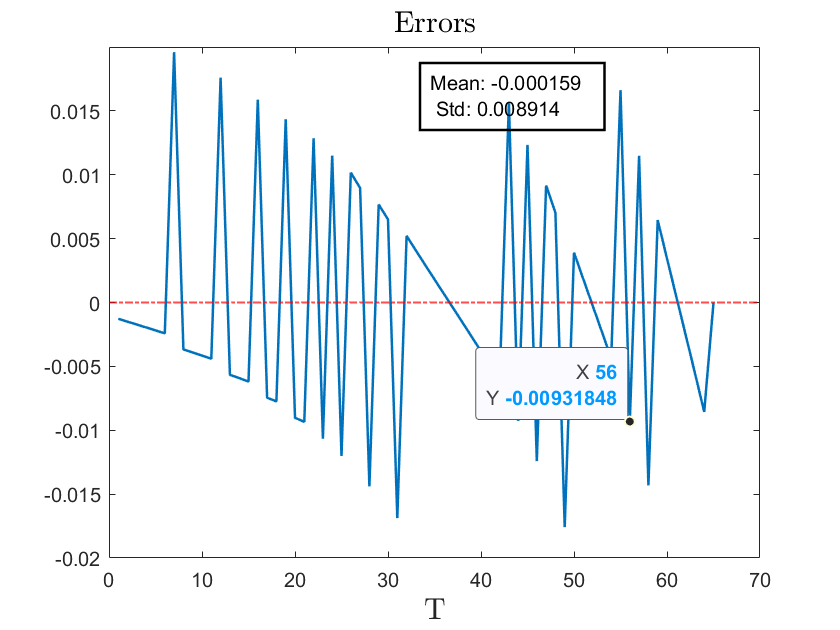
\includegraphics[width=\maxwidth{56.196688409433015em}]{figure0.png}
\end{center}

\begin{par}
\begin{flushleft}
Como podemos notar, los errores toman una forma en zigzag, que oscila alrededor del cero. En el último periodo de hecho sabemos que $e_T \;\mathrm{donde}\;T\;\mathrm{es}\;\mathrm{el}\;\mathrm{último}\;\mathrm{periodo}$ es cero, dado lo que comentamos inicialmente: en este no tenemos error en la predicción: sabemos que consumimos todo. Mientras nos devolvemos en el tiempo, los errores se van moviendo sin una tendencia clara. A vecs hay una sobrestimación, y a veces una subestimación. De hecho, el valor esperado de ese error es cercano a cero y su desviación estándar es muy baja notando que sus valores extremos positivos y negativos coinciden, reflejando que esta distribución es bastante simétrica (ver el cuadro).
\end{flushleft}
\end{par}

\begin{par}
\begin{flushleft}
Ahora bien, hay dos puntos que destacar. El primero tiene que ver con que en algunos periodos pareciera que el error se mantiene constante. Eso sería un error de interpretación. Más bien lo que tenemos es que, dado que tenemos pocos periodos y el horizonte de tiempo no es continuo, la transición de un periodo a otro es visible (véase por ejemplo cuando se pasa del periodo 10 al 11).  El segundo periodo tiene que ver con la cantidad de activos que tenemos para hacer la estimación sobre la trayectoria del consumo. Recordemos que pensamos este problema en términos de funciones continuas y diferenciables (suavizamiento del consumo), pero al construir grillas de activos discretizamos el problema. Con ello, tanto las decisiones óptimas (que podemos ver en las policy functions) como los errores de estimación asociado a esas condiciones óptimas, no se verán continuas. Discutiremos este elemento y sus implicancias en los errores de estimación en el siguiente punto. 
\end{flushleft}
\end{par}

\matlabheadingthree{(c) Repetir el proceso con una grilla de activos A, de 5001. Verifique que la grilla contiene el cero. ¿Cómo cambian los resultados del ítem anterior?}

\begin{par}
\hfill \break
\end{par}

\begin{matlabcode}
%% Consumo en el ciclo de vida con mas grilla - item (c)
clc; clear; 

%Parameters
T =65; 
beta = 0.96; 
sigma = 2; 
r = 0.04; 
liq = 100;
A = linspace(-15,25,5001)'; % Tienen como deuda maxima -15 y ahorro 25
% Si mi restriccion de liquidez es b = 100 no es activo

%Wage as function and vector
Z  = @(t) 1.25 + 6e-2*t - 1e-3*t.^2; % se multiplica escalar, entonces voy a ocupar vectores
w = Z(1:T); % evaluar desde 1 hasta t
w_mean = mean(w)*ones(1,T); % ones es para hacer un vector de la media

%Value function iteration
tic
[Vt,At,Ct,Ap,Am,Cm] = value_matriz(T,beta,sigma,r,A,Z,liq);
toc
\end{matlabcode}
\begin{matlaboutput}
Elapsed time is 16.295086 seconds.
\end{matlaboutput}

\begin{par}
\begin{flushleft}
Calculando errores
\end{flushleft}
\end{par}

\begin{matlabcode}
constant=(beta*(1+r))^(-1/sigma);
errors=zeros(1,T);
for k=1:T-1    
    errors(k)=constant*(Ct(k+1))/Ct(k)-1;
end
\end{matlabcode}

\begin{par}
\begin{flushleft}
Ahora si graficamos la relación
\end{flushleft}
\end{par}

\begin{matlabcode}
tx= {'Interpreter','Latex','FontSize', 15};
meanVal = mean(errors);
stdVal = std(errors);
str = sprintf('Mean: %f\n Std: %f',meanVal,stdVal);

figure(2)
plot(1:T, errors(:,1:end))
yline(0,'LineStyle','-.','Label','','Color','red','LabelVerticalAlignment','middle','LabelHorizontalAlignment','center','LineWidth',1)
xlabel('T',tx{:})
title('Errors',tx{:},'FontSize', 15)
annotation("textbox",[.5 .5 .4 .4], 'String',str,'FitBoxToText','on' )
\end{matlabcode}
\begin{center}
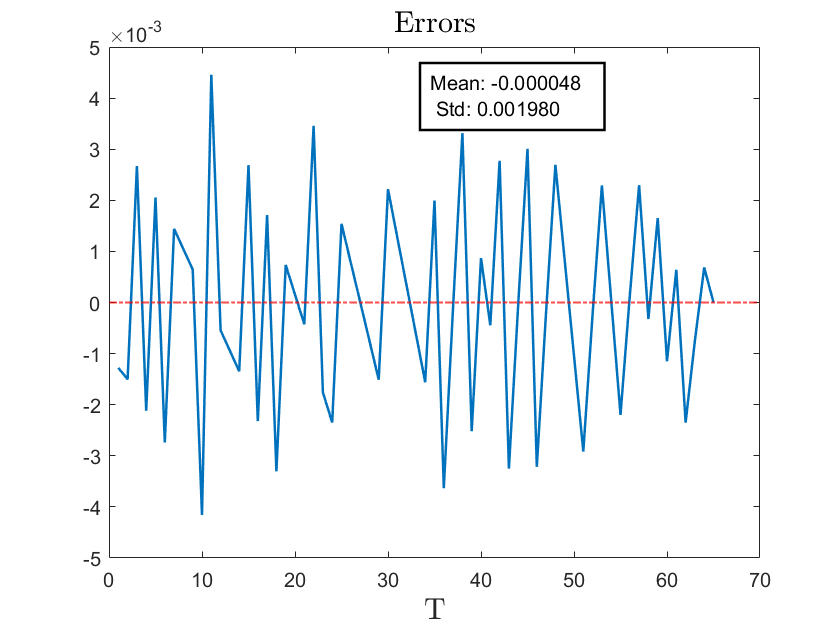
\includegraphics[width=\maxwidth{56.196688409433015em}]{figure1.png}
\end{center}

\begin{par}
\begin{flushleft}
La interpretación ya la habíamos enunciado, pero ahora la fomalizaremos. En concreto, al aumentar el número de celdas de la grilla de activos, estamos permitiendo que el agente tenga más posibilidades de decisión en un intervalo de consumo factible (cumpliendo con las condiciones de no negatividad y condición de transversalidad o esquemas de no ponzi). Al conseguir esto, podremos modelar de manera \textbf{más precisa qué pasaría con el consumo de un t}, dada una tasa de interés e impaciencia. La razón es que la decisión óptima del agente respecto al ahorro y consumo podrá ser obtenida no solo con 1001 posibilidades de distribución de activos (sujeto a las restricciones), sino que 5001 posibilidades de distribución de activos en el tiempo. 
\end{flushleft}
\end{par}

\begin{par}
\begin{flushleft}
Pongamos un ejemplo burdo para que quede más claro. Imaginemos que antes determinabamos el comportamiento del agente con dos activos probables entre [-15 y 25], es decir, o es -15 o 25. En función de eso, sabemos que el agente en el último periodo no puede morir con deuda entonces, en el último periodo tiene 25 de activos para consumir  (y se lo consume todo en el último periodo, no dejando nada para el consumo de mañana), o tiene una deuda de -15 en el último periodo y decide no consumir nada en el último periodo para no morir con deuda, es decir, consumiendo en el primer periodo todo (aunque sabemos que no sería un caso factible si no tenemos ingresos que hagan 0 ese nivel inicial de activos).  Con ello, estamos llegando a una relación muy poco precisa sobre la relación del consumo en el último periodo y el penúltimo. 
\end{flushleft}
\end{par}

\begin{par}
\begin{flushleft}
¿Qué pasa si agregamos una posibilidad intermedia?, o en otras palabras ¿Si entre -15 y 25 tenemos ahora 3 posibilidades te tenencia de activos. Entonces podremos conocer mejor cómo se comportaría el agente bajo esa circunstancia (por ejemplo, tener 10 de activos). Estaremos más cerca de conocer cómo el agente decide en el óptimo como suavizar su consumo. Así mismo, si aumentamos las distintas posibilidades de activos posibles, podremos entender de manera "más continua" ese comportamiento. Así, entonces, evidentemente los errores de estimación en cada momento del tiempo disminuirán (como se ve en la gráfica, en promedio son mucho más cercanos a cero), sus valores máximos y mínimos son más pequeños que en ejemplo anterior, y su desviación estándar también (se concenta más en el cero). Es decir, a medida que tengo más información sobre esta variable de estado (inicialmente) y de control (cuando miramos el periodo siguiente, resolviendo de atrás en adelante), puedo obtener un mayor grado de precisión sobre cómo se suaviza el consumo. 
\end{flushleft}
\end{par}

\end{document}
